% Условная компиляция для самостоятельной работы
\ifdefined\mainfile
    % Если это часть основного файла, не добавляем начало и конец документа
\else
    \documentclass[12pt, a4paper]{report}
    \usepackage{/Users/vladbelousov/Desktop/Semestr_4-FP-NSU/Настройка/library}
    \usepackage[utf8]{inputenc} % Подключение поддержки UTF-8
    \begin{document}
\fi

%%-------------------------------%%

\section{Связь комплексной степени когерентности и спектральной плотности энергии волнового поля} 

\[\kern-1cm G_{11}^{(0)} = \lim_{T  \to \infty} \frac{1}{T }  \int_{-\frac{T}{2 } }^{\frac{T}{2 }  } E_1(t ) E_1 ^{* }  (t +\Delta t ) dt = \frac{1}{T }  \int_{-\frac{T}{2 } }^{\frac{T}{2 } } dt \frac{1}{\sqrt{2 \pi } } \int_{-\infty}^{\infty} E_1 (\omega ) e^{ - i \omega t } d \omega    \frac{1}{\sqrt{2 \pi } } \int_{-\infty}^{\infty} E_1 ^{* }  (\omega ' ) e^{i \omega (t + \Delta t )} d \omega ' =        \] 
\[ = \frac{1}{2 \pi T } \int  d \omega \int d \omega ' E_1 ( \omega ) E_1 ^{* }  (\omega ' ) e^{i \omega ' \Delta t } \int_{-\infty}^{\infty} dt e^{- i (\omega - \omega'  )t} = \frac{1}{T }  \int_{-\infty}^{\infty} d \omega' |E_1 (\omega' )| ^2 e^{ i \omega ' \Delta t } = \left[ \omega' = -\omega \right]    = \] 
\[  =\frac{\sqrt{2 \pi } } {T } \frac{1}{\sqrt{2 \pi } } \underbrace{\int_{-\infty}^{\infty} |E_1(\omega )| ^2 e^{ - i \omega \Delta t } d \omega}_{(*)}   \] 
, где \( (*) \)  - обратное преобразование Фурье-преобразования от спектральной плотности энергии.

\[ \gamma_{11}^{(0 )}   (\Delta t ) = \frac{ G_{11} ^{(0 )} (\Delta t )}{G_{11}^{(0 )}  (0 )}= \frac{\displaystyle  \frac{1}{\sqrt{ 2 \pi } } \int_{-\infty}^{\infty} |E_1 (\omega )| ^2 e^{ - i \omega \Delta t }d \omega  }{\displaystyle  \frac{1}{ \sqrt{2 \pi }} \int_{-\infty}^{\infty} |E_1 (\omega )| ^2 d \omega }   \] 

\[ I = I_1 + I_2 + 2 \sqrt{I_1 I_2 } \mathrm{Re }  \left( \gamma_{11} ^{ (0 )} \left( \frac{\Delta r }{c}  \right) \right)   \] 

\[ |E_1 (\omega)| ^2 = \frac{A}{(\omega - \omega_0 ) ^2 + \gamma ^2 }   \]
- лоренцевский профиль \( \to  \) спектральная плотность энергии скопления спонтанно излучающих атомов. 

\[ \int_{-\infty}^{\infty} \frac{A e^{ - i \omega \Delta t }d \omega         }{(\omega - \omega_0 ) ^2 + \gamma ^2 }  \] 

\begin{center}
    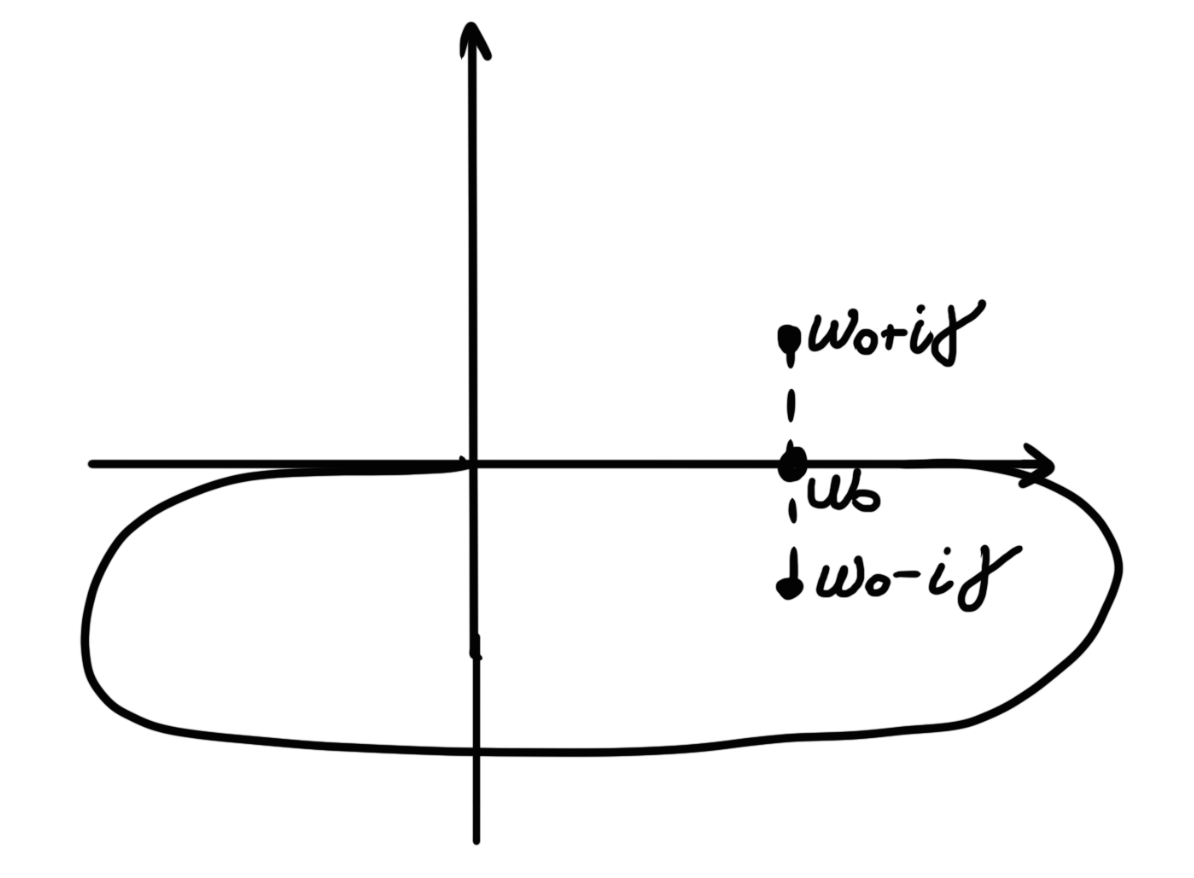
\includegraphics[width=0.4\textwidth]{/Users/vladbelousov/Desktop/Semestr_4-FP-NSU/ЭиО/Лекции_по_дням/image/111.png}
\end{center}

В верхней полуплоскости \( \omega = \omega '+ i \omega '' \text{ }  (\omega '' > 0 ) \). Интегрируем в нижней полуплоскости \( (\Delta t > 0) \): 

\[ e^{- i \omega \Delta t + \omega '' \Delta t } ( \omega'' < 0)  \] 

\[ Int = - A \frac{ 2 \pi i }{- 2 \omega \gamma } e^{ - i (\omega_0 - i \gamma ) \Delta t } = \frac{\pi A }{\gamma } e^{ - i \omega_0 \Delta t } e^{ - \gamma \Delta t }      \] 

Схема Юнга с одинаковыми щелями  (точечный источник) \( I_1 = I_2 = I_0 \Rightarrow  \) 

\[ I = 2 I_0 \left( 1 + e ^{ - \gamma \frac{\Delta r }{c } } \cos \left( \omega_0 \frac{\Delta r }{c }  \right) \right) \]

\begin{center}
    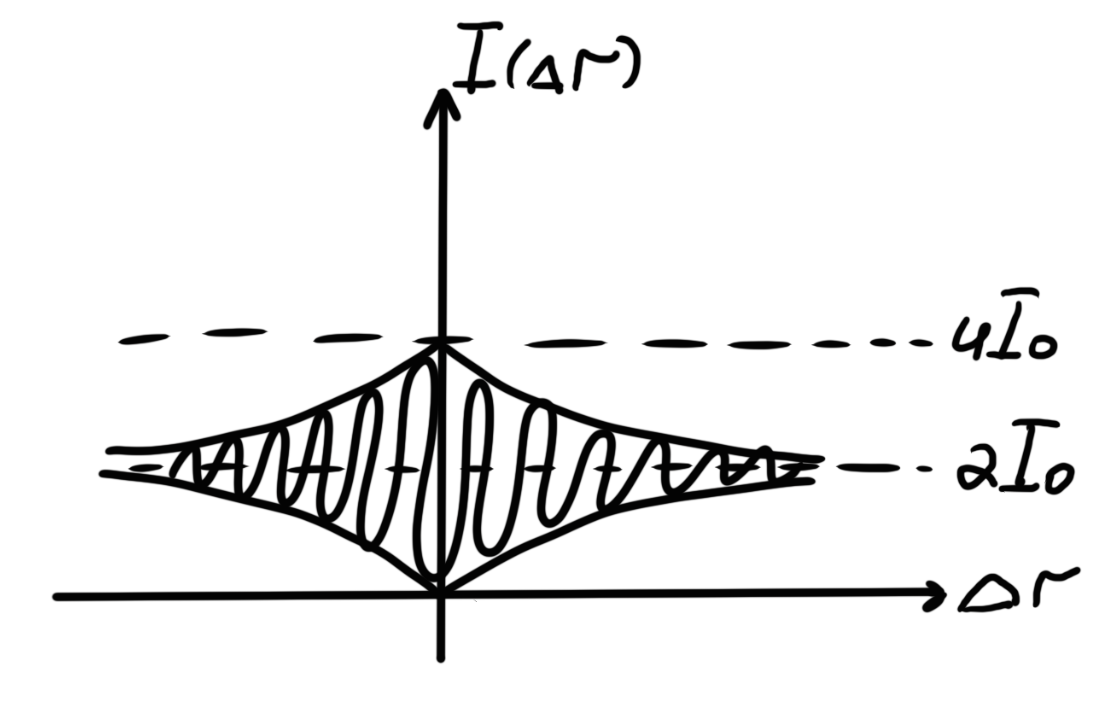
\includegraphics[width=0.5\textwidth]{/Users/vladbelousov/Desktop/Semestr_4-FP-NSU/ЭиО/Лекции_по_дням/image/112.png}
\end{center}

\[ V = e^{ - \gamma \frac{ x d }{L} }  \] 

\section{Апертура интерференции}

\begin{center}
    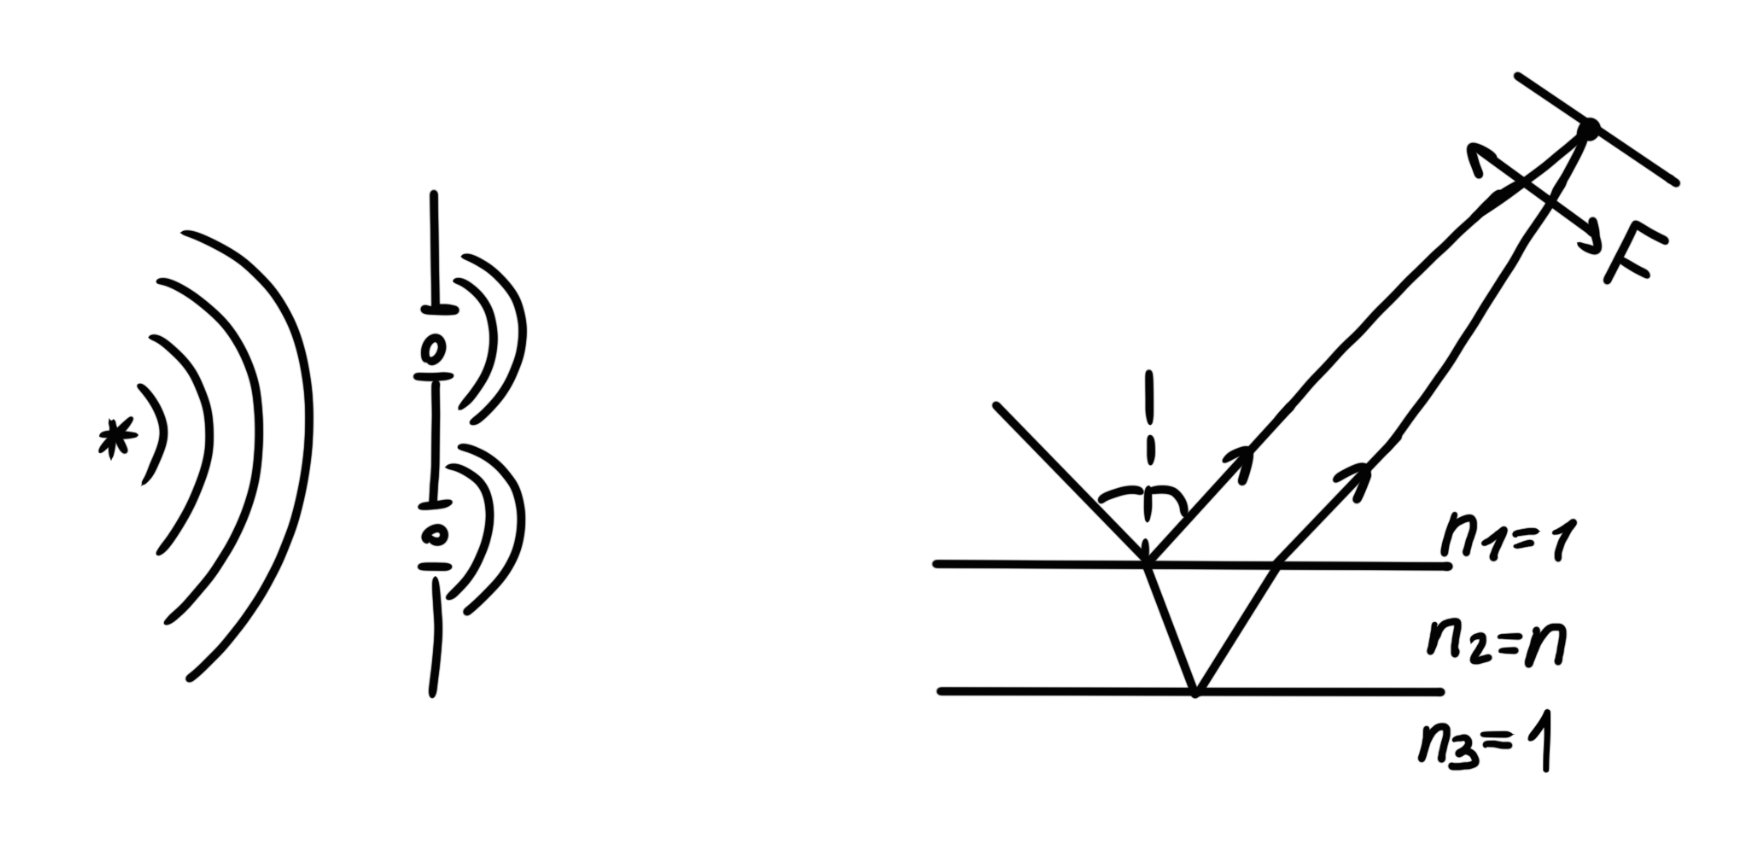
\includegraphics[width=0.5\textwidth]{/Users/vladbelousov/Desktop/Semestr_4-FP-NSU/ЭиО/Лекции_по_дням/image/113.png}
\end{center}
Интерферируют поля разных частей волнового фронта. 

\begin{center}
    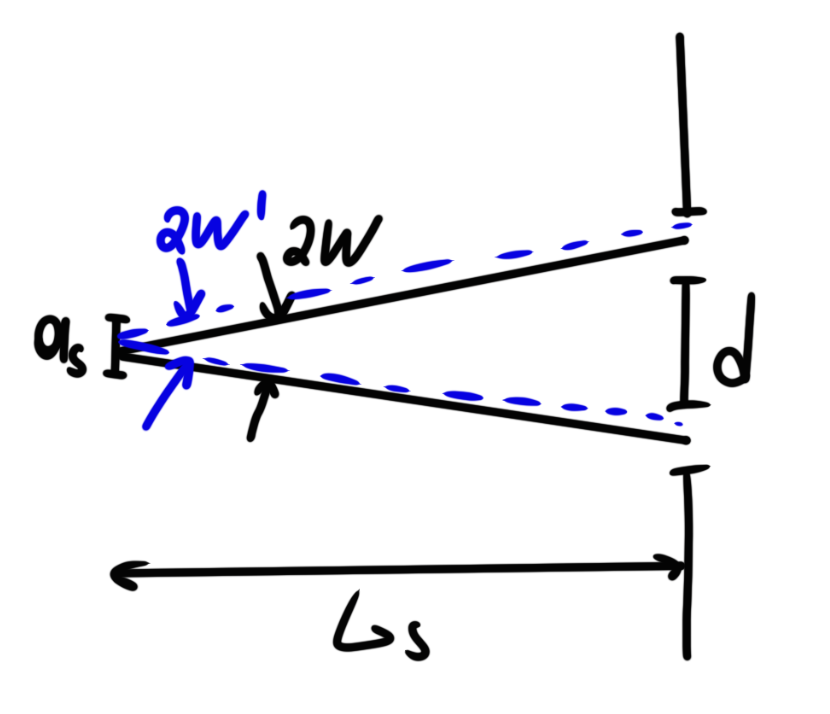
\includegraphics[width=0.3\textwidth]{/Users/vladbelousov/Desktop/Semestr_4-FP-NSU/ЭиО/Лекции_по_дням/image/114.png}
\end{center}
Схема деления амплитуды волны: 

\[ d < l_1 = \frac{\lambda}{2 \theta_s } = \frac{\lambda}{\displaystyle \frac{2a_s}{L_s} }  \left( V>\frac{1}{2}  \right) \] 

Перепишем это соотношение в ином виде, пригодном и для схем деления амплитуды волны: 

\begin{center}
    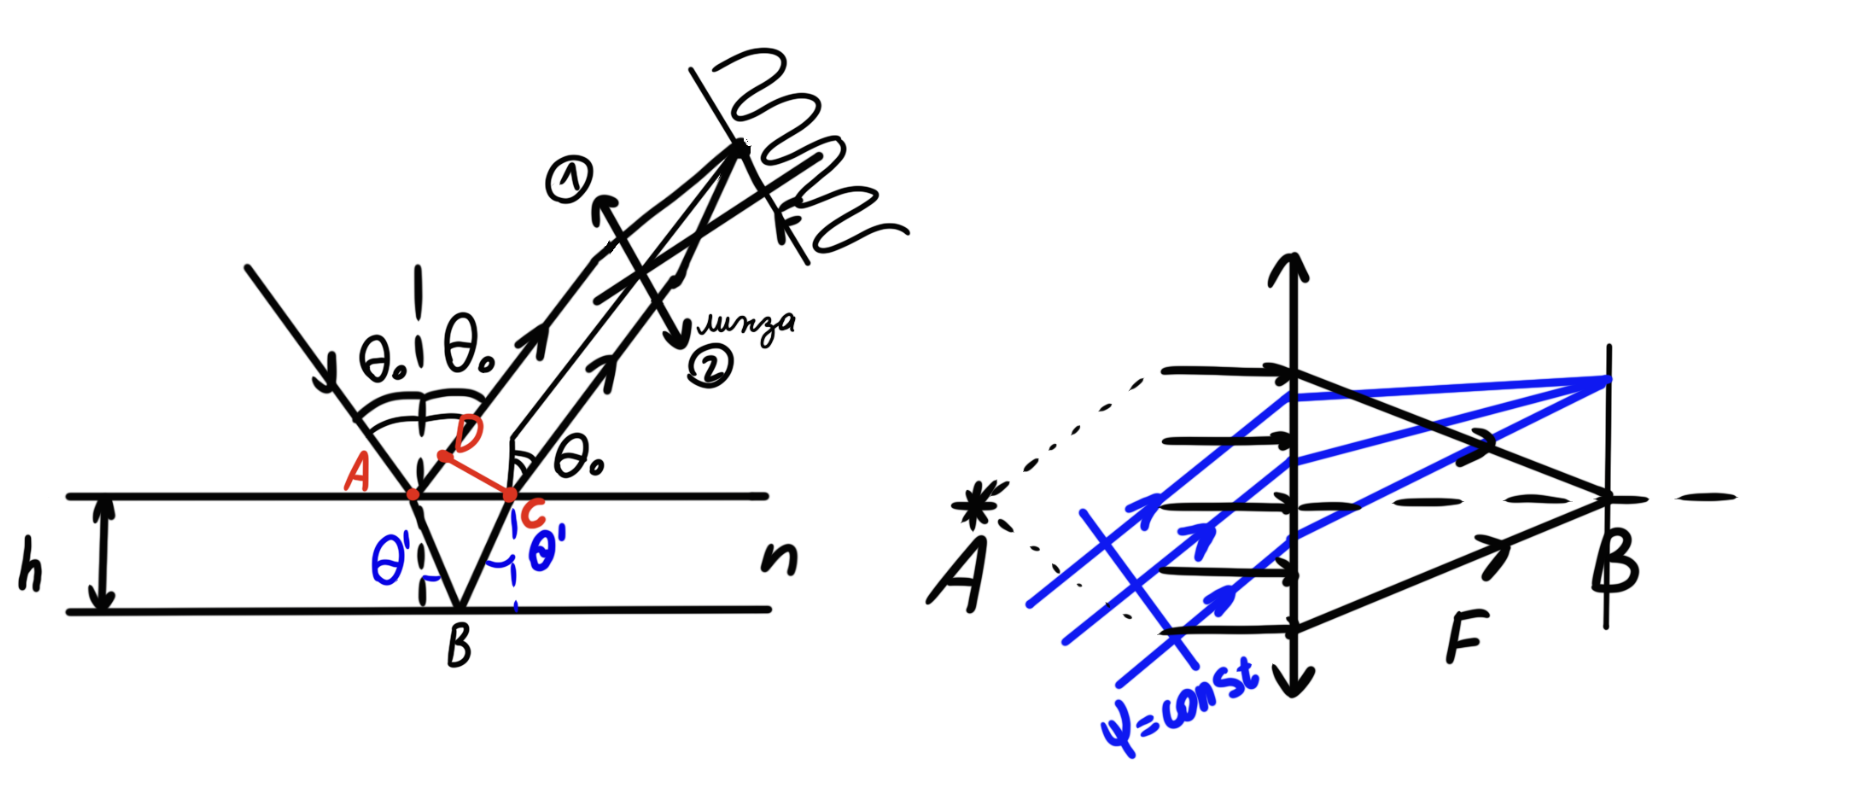
\includegraphics[width=0.7\textwidth]{/Users/vladbelousov/Desktop/Semestr_4-FP-NSU/ЭиО/Лекции_по_дням/image/115.png}
\end{center}
, где \( 2 w  \) - апертура интерференции. В параксиальном приближении \( (a_s , d ,x ,y ) \ll L, L_s : \text{ }  2 w \approx 2 w ' \) 

\[ 2 w = \frac{d}{L_s } \quad  d \le \frac{\lambda L_s}{2 a_{s} } \quad  w a_{s_{\perp } }  <    \frac{\lambda}{4} \] 
, где \( a_{s_{ \perp } }  \) - поперечный размер протяженного источника по отношению к направлению на щели. 

\section{Интерференция в тонких пленках}

Плоскопараллельная пластина. Локализация полос на \( \infty  \). 

\begin{center}
    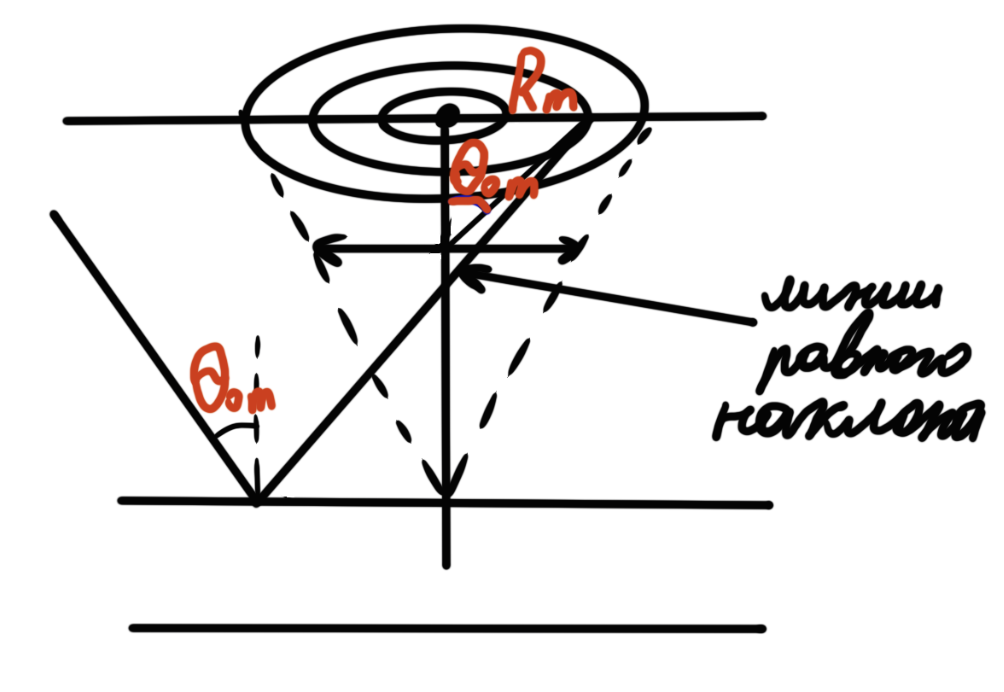
\includegraphics[width=0.5\textwidth]{/Users/vladbelousov/Desktop/Semestr_4-FP-NSU/ЭиО/Лекции_по_дням/image/116.png}
\end{center}
\( A \) и \( B \) - сопряженные точки.

\( \int n d S  \) вдоль всех лучей из точки \( A \) в точку \( B \)  (сопряженную к \( A \)) \( = \mathrm{cosnt}   \) 

\( \Delta r  \)  - разница оптических путей пучков. 

(1) и (2) = 2 \( |AB|n - \displaystyle  |AD| + \frac{\lambda_0}{2}  \) (отражение от более плотной оптической среды)

\[ |AB | = \frac{h}{\cos \theta' } \quad  |AD| = 2 h \text{ } \mathrm{ tg}   \theta ' \sin  \theta_0 \]  

\[  n \sin \theta ' = \sin \theta_0  \] 
\[ \Delta r = \frac{2hn}{\cos \theta ' }- 2h \frac{\sin  \theta ' n \sin \theta ' }{\cos \theta ' } \frac{\lambda_0}{2 }  = \frac{2hn}{\cos  \theta' } (1 - \sin  ^2 \theta ' ) \frac{\lambda_0}{2 }  = 2hn \cos \theta ' + \frac{\lambda_0}{2 }  = 2hn \sqrt{1 - \sin  ^2 \theta ' }   + \frac{\lambda_0}{2 }   \] 
\[ \Delta r = 2 h \sqrt{n ^2 - \sin  ^2 \theta_0 } + \frac{\lambda_0}{2 }  \] 

Пусть ось линзы \( \perp   \) пластине: 

\begin{center}
    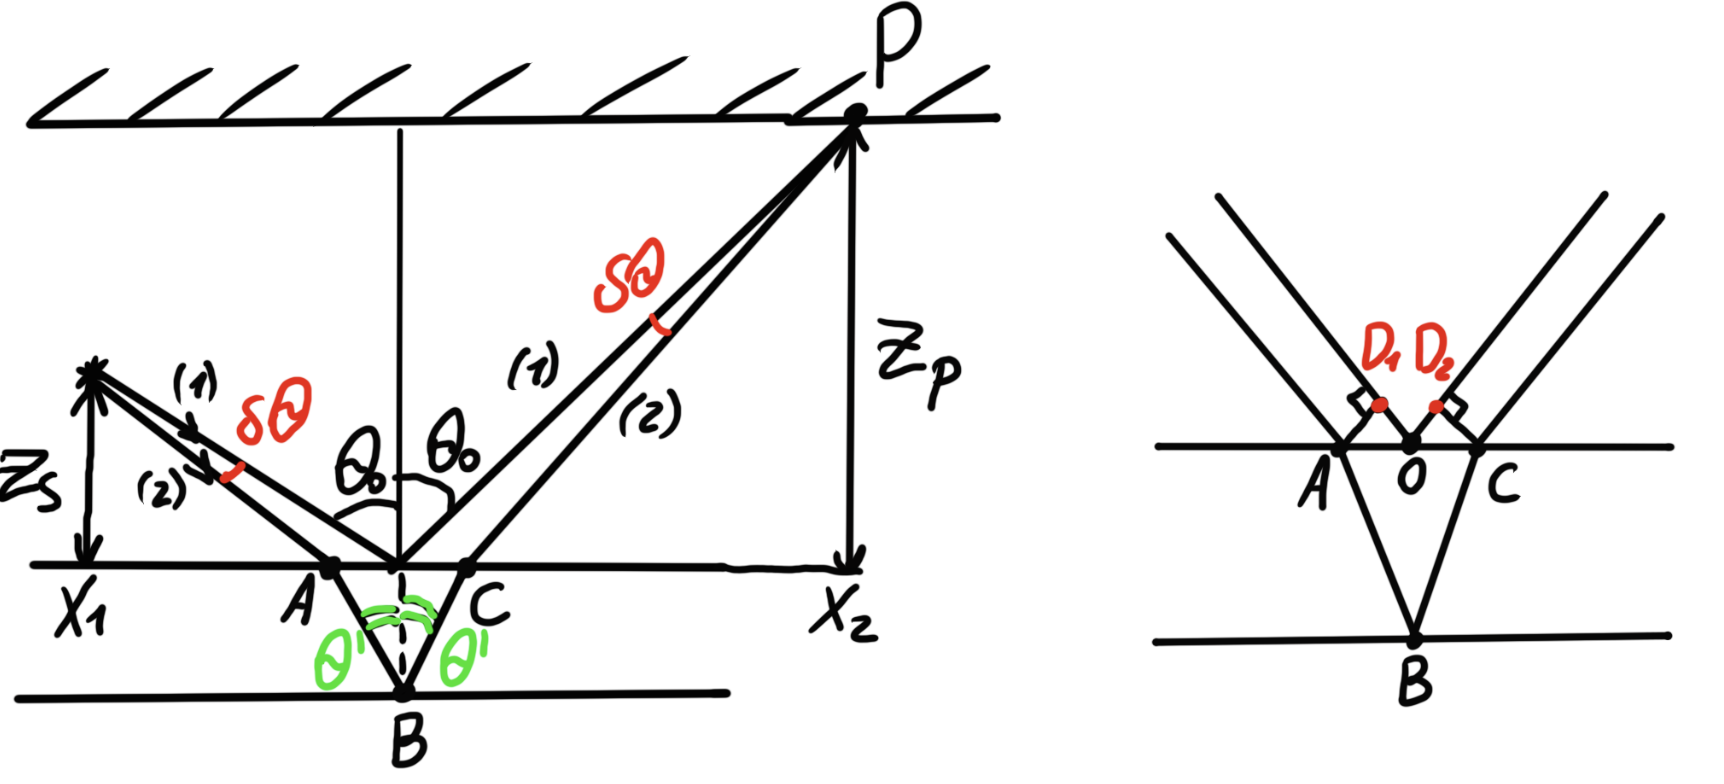
\includegraphics[width=0.7\textwidth]{/Users/vladbelousov/Desktop/Semestr_4-FP-NSU/ЭиО/Лекции_по_дням/image/117.png}
\end{center}

\[ 2 h \sqrt{n ^2 - \sin  ^2 \theta_{0m }  } + \frac{\lambda_0}{2 }  = m \lambda_0 , \text{ }  m \text{ - целое}  \] 
\[ R_m = F \theta_{0m}  \] 

Это интерференционная картина локализована на бесконечности, может наблюдаться в фокальной плоскости линзы или аккомодированным на \( \infty  \) глазом. \( w a_{s_{\perp } } < \displaystyle \frac{\lambda}{4}   \). В нашем случае интерферируют параллельные лучи \( \Rightarrow w = 0 \Rightarrow a_{s _{\perp  } }   \) может быть очень большим.

\textbf{Опыт Поля} 

%img

\[ \Delta r = n \left( |AB| + |BC| \right) - |O D_1     |- |O D_2   | + \frac{\lambda_0}{2 }  \] 

\[ \sin (\theta_0 - \delta \theta  )  = n \sin \theta' \text{ при }  \Delta \theta \ll \theta_0 \Rightarrow \sin \theta_0 \approx n \sin \theta'  \] 

\[ |x_1 x_2 | = z_s \mathrm{tg }  \theta_0 + z_p \mathrm{tg }   \theta_0 = (z_s + z_p ) \mathrm{tg }  (\theta_0 - \delta \theta ) + h \mathrm{tg }  \theta ' 2     \] 
\[ \Rightarrow (z_s + z_p )(\mathrm{tg }  \theta_0 - \mathrm{tg }  (\theta_0 - \delta \theta )  ) = 2h \frac{\sin \theta_0 }{n \sqrt{\displaystyle  1 - \frac{\sin  ^2 \theta_0 }{n ^2 } }} \] 

\[ \delta \theta = \frac{2h}{(z_s +z_p )} \frac{\sin  \theta_0 \cos  ^2 \theta_0 }{\sqrt{n ^2 - \sin  ^2 \theta_0 }} \ll 1    \] 
, где \( \delta \theta  = 2w \)  - апертура интерференции.



%%-------------------------------%%

% Закрытие документа, если файл компилируется отдельно
\ifdefined\mainfile
    % Если это основной файл, не нужно заканчивать документ
\else
    \end{document}
\fi